%\section{Une section}

% remarque : pour qu'un mot se retrouve dans le lexique : \MotDefinition{asymptote horizontale}{} 

\begin{aconnaitre}
Deux grandeurs sont \textbf{proportionnelles} lorsque l’une s’obtient en multipliant (ou en divisant) l’autre par un même nombre non nul.

Ce coefficient multiplicateur est un \MotDefinition{coefficient de proportionnalité}{}.
\end{aconnaitre}

\begin{methode*1}[Trouver le coefficient de proportionnalité]

 \begin{exemple*1}
Le carburant pour un motoculteur est un mélange de super et d’huile où les doses d’huile et d’essence sont proportionnelles : il faut 2 doses d’huile pour 3 doses de super. Détermine le coefficient de proportionnalité qui permet d’obtenir la dose de super en fonction de la dose d’huile.
\begin{center} 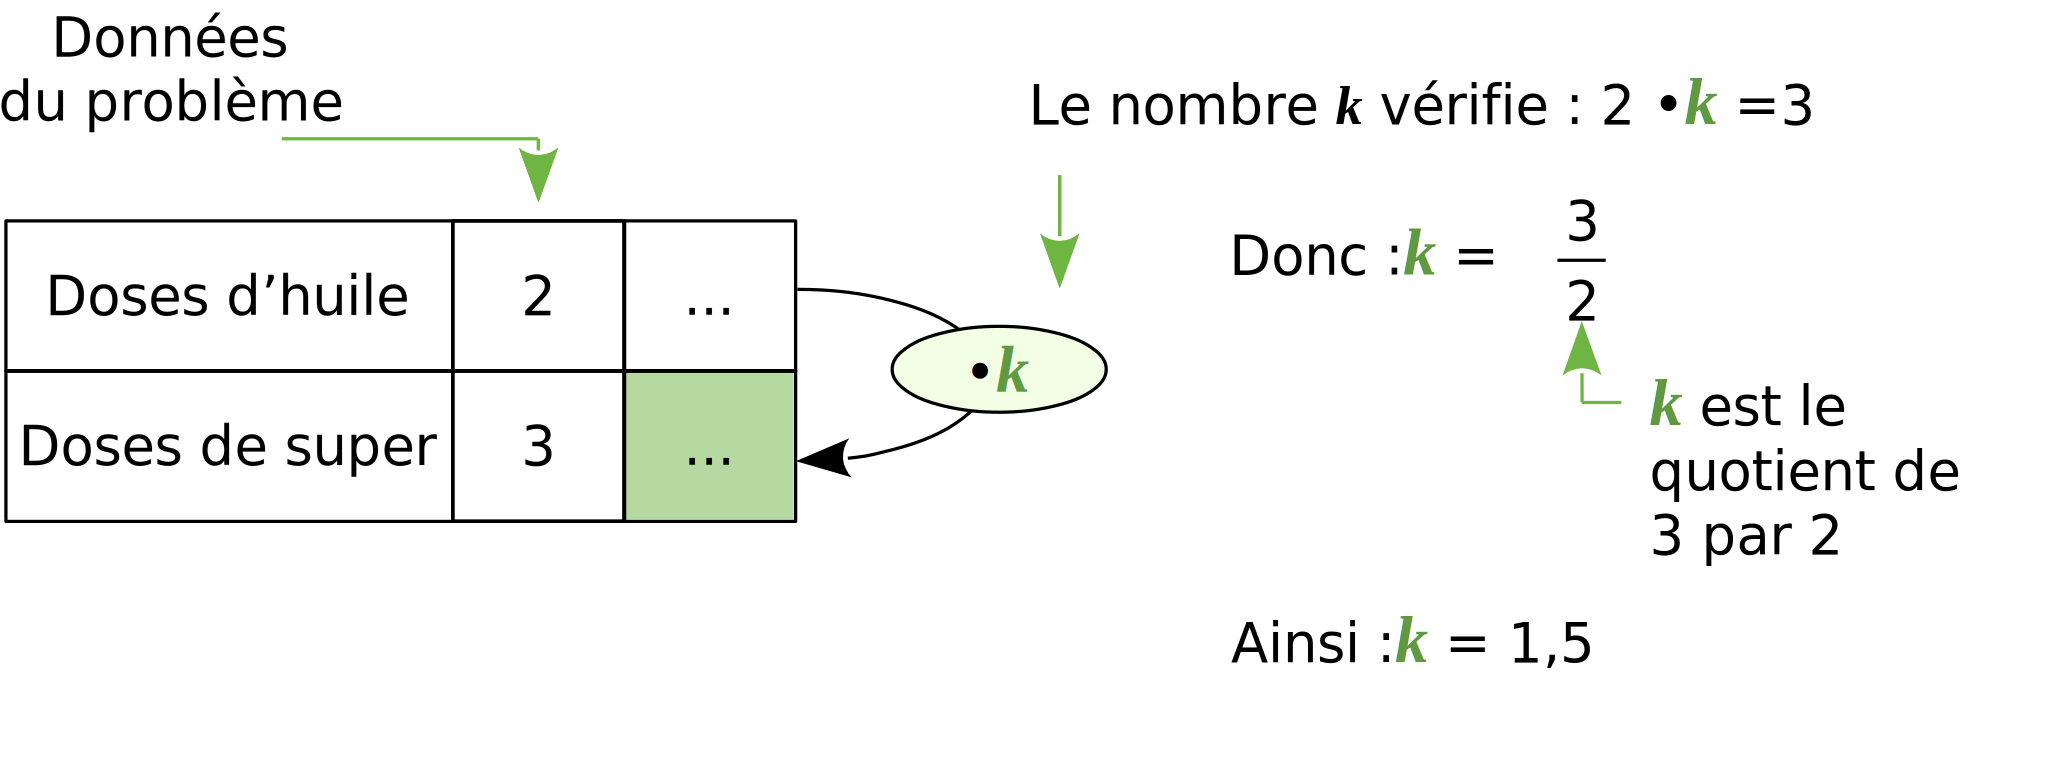
\includegraphics[width=12cm]{probleme_propor1} \end{center}
Le coefficient de proportionnalité qui permet d'obtenir la dose de super en fonction de la dose d'huile est 1,5.
 \end{exemple*1}

 \begin{remarque}
Soit $\textbf{\textcolor{C2}{h}}$ le coefficient de proportionnalité qui permet d'obtenir la dose d’huile en fonction de la dose de super :
\begin{center} 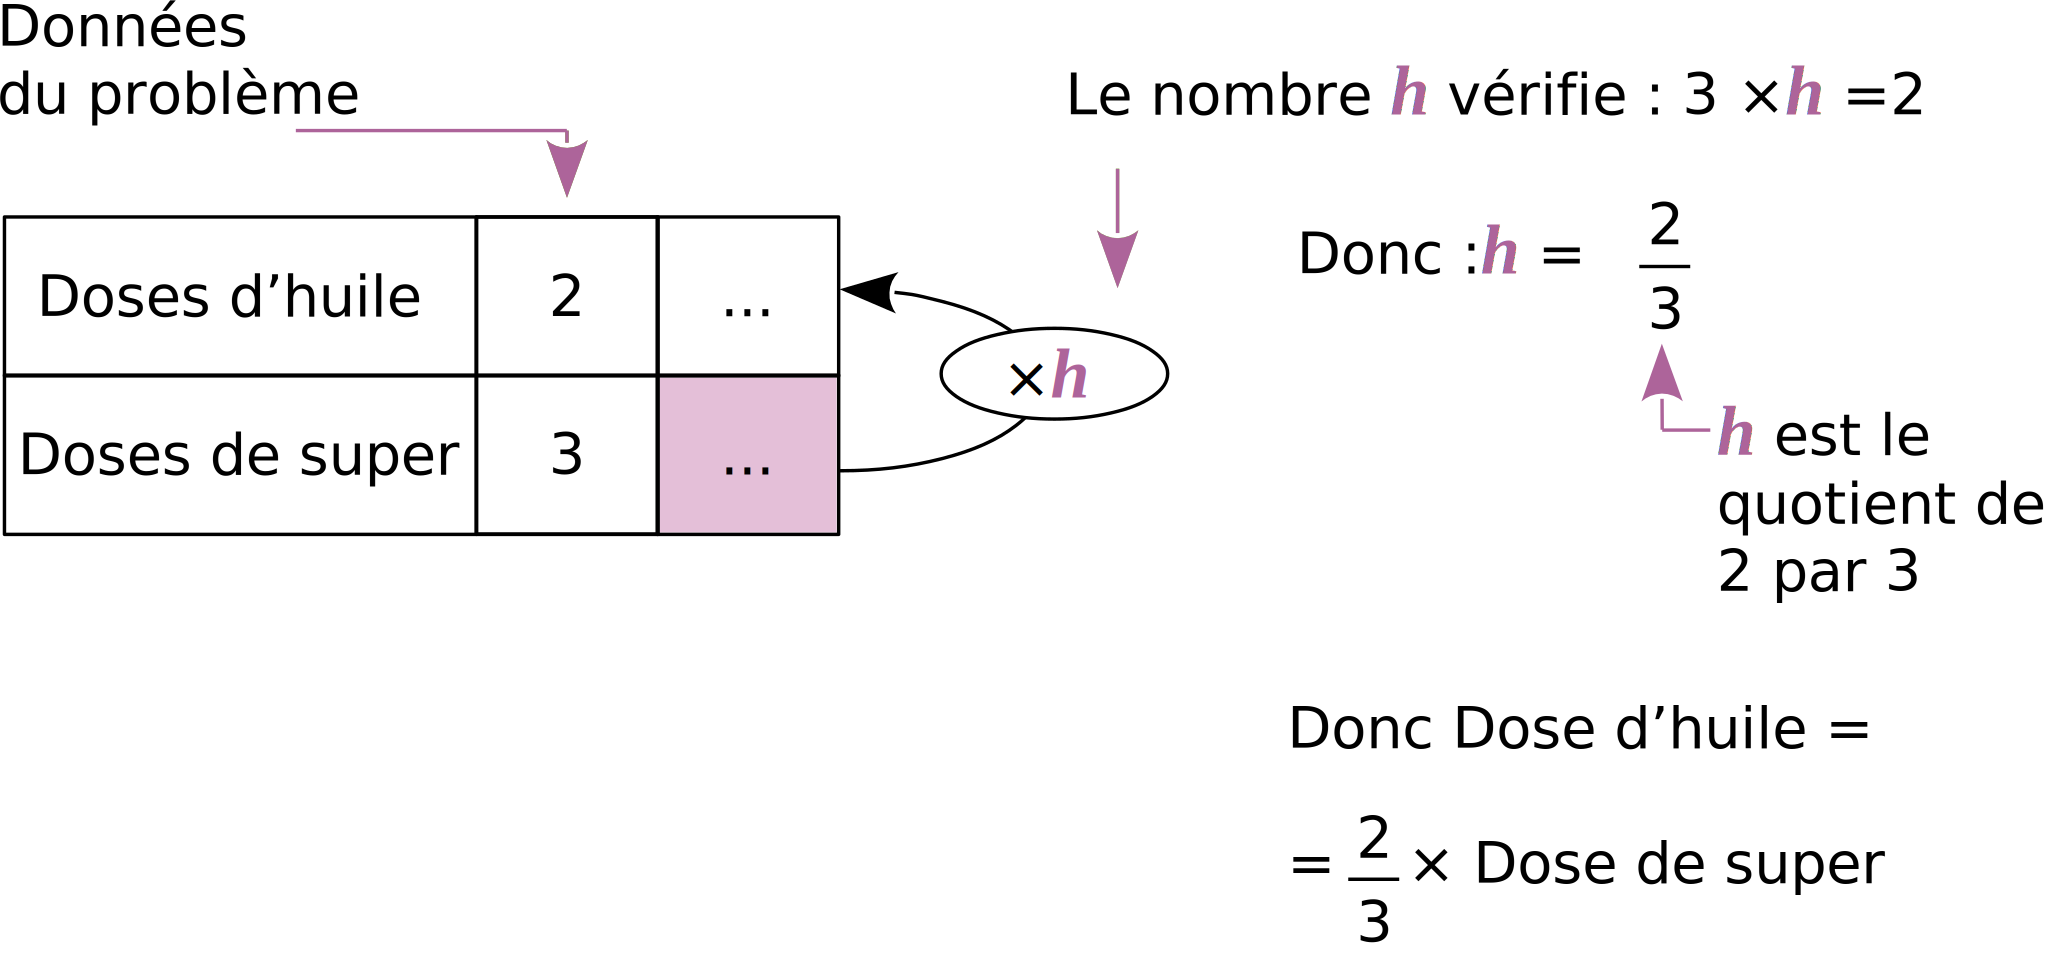
\includegraphics[width=12cm]{probleme_propor2} \end{center}
 \end{remarque}

 \exercice  
Un magasin vend 2 kg de pommes pour 5 CHF. Par quel nombre faut-il multiplier le nombre de kg de pommes pour obtenir celui du prix ?
%\correction

 \end{methode*1}
 
 %%%%%%%%%%%%%%%%%%%%%%%%%%%%%%%%%%%%%%%%%%%%%%%%%%%%%%%%%%%%%%%%%%%%%%%%
 
 \begin{aconnaitre}
Pour vérifier si deux grandeurs sont \MotDefinition{proportionnelles}{}, on doit s’assurer qu’elles évoluent toutes les deux dans les mêmes proportions.
\end{aconnaitre}

\begin{methode*1}[Identifier une situation de proportionnalité]

 \begin{exemple*1}
Les tarifs des remontées mécaniques d’une station de ski sont les suivants : 50 CHF la journée, 90 CHF les deux jours et 240 CHF les 6 jours. Le prix à payer est-il proportionnel à la durée ? \\[1em]
Si le prix à payer était proportionnel à la durée, en payant 50 CHF la journée, on devrait payer le double pour deux jours, soit 100 CHF et 6 fois plus pour six jours, soit 300 CHF. \\[0.5em]
Comme ce n'est pas le cas, le prix à payer n'est pas proportionnel à la durée. 
 \end{exemple*1}

 \exercice  
Un commerçant vend ses croissants à 0,65 CHF l’unité ou à 5,00 CHF le paquet de 10. Cette situation ne relève pas d’une situation de proportionnalité. Explique pourquoi.
%\correction

 \end{methode*1}
 
 %%%%%%%%%%%%%%%%%%%%%%%%%%%%%%%%%%%%%%%%%%%%%%%%%%%%%%%%%%%%%%%%%%%%%%%%

\begin{methode*1}[Utiliser les propriétés de la proportionnalité]

 \begin{exemple*1}
Complète le tableau de proportionnalité suivant :
\begin{center}
\begin{tabularx}{0.8\linewidth}{|c|*{6}{>{\centering\arraybackslash}X|}}
\hline
\cellcolor{C4} Masse de pommes (en kg) & 16 & 8 & 2 & & 24 \\ \hline
\cellcolor{C4} Prix (en CHF) & & 7,8 & & 78 &  \\ \hline
  \end{tabularx}
 \end{center}
\begin{center} 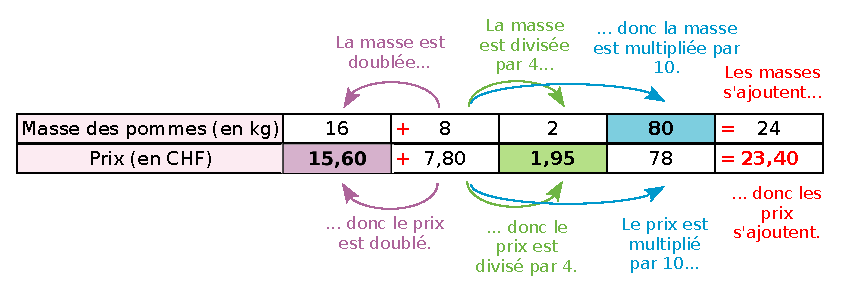
\includegraphics[width=12.5cm]{prix_pommes} \end{center}
 \end{exemple*1}


 \exercice  
La voiture de Marie consomme 4,5 l d'essence sur 100 km :
\begin{enumerate}
 \item Quelle sera sa consommation si elle parcourt 150 km ? 250 km ? 1 250 km ?
 \item La voiture de Marie a consommé 13,5 l d'essence. Quelle distance a‑t‑elle parcourue ? Quelle distance peut-elle parcourir avec 135 l d'essence ?
 \end{enumerate}
%\correction

 \end{methode*1}
 
 %%%%%%%%%%%%%%%%%%%%%%%%%%%%%%%%%%%%%%%%%%%%%%%%%%%%%%%%%%%%%%%%%%%%%%%%


\begin{methode*1}[Calculer avec un cœfficient de proportionnalité]

 \begin{exemple*1}
Lucie paye 100 CHF pour acheter 20 clés. Quelle est le nombre de clés qu'elle peut acheter pour 55 CHF ? Et pour 30 CHF ? Si elle désire acheter 126 clés, Combien devra-t-elle payer ? \\[1em]
Le nombre de clés est proportionnel au prix. \\[0.5em]
\begin{minipage}[c]{0.08\linewidth}
 
\includegraphics[width=1.1cm]{mult_02}
 \end{minipage} \hfill%
 \begin{minipage}[c]{0.8\linewidth}
\begin{tabularx}{\linewidth}{|c|*{4}{>{\centering\arraybackslash}X|}}
\hline
\cellcolor{C4} Coût (en CHF) & 100 & 55 & 30 & \textcolor{B2}{\textbf{630}} \\\hline
\cellcolor{C4} Nombre de clés & 20 &  \textcolor{A2}{\textbf{11}} &  \textcolor{A2}{\textbf{6}} & 126 \\\hline
  \end{tabularx}
  \end{minipage} \hfill%
  \begin{minipage}[c]{0.08\linewidth}
   
\includegraphics[width=1.1cm]{div_02}
   \end{minipage} \\ 
\begin{itemize}
 \item On calcule le coefficient \textbf{de proportionnalité} : $20 : 100 =$ \textcolor{A2}{\textbf{0,2}}.
 \item Pour trouver les nombres de la 2\up{e} ligne du tableau, on multiplie les nombres de la 1\up{re} ligne par le coefficient de proportionnalité. Pour trouver les nombres de la 1\up{re} ligne du tableau, on divise les nombres de la 2\up{e} ligne par le coefficient de proportionnalité.
  \end{itemize}
 \end{exemple*1}


 \exercice
Complète le tableau de proportionnalité suivant :
\begin{center}
\begin{tabularx}{0.9\linewidth}{|c|*{5}{>{\centering\arraybackslash}X|}}
\hline
\cellcolor{C4} Nombre de personnes & 7 & 13 & 5 & & \\\hline
\cellcolor{C4} Prix payé pour entrer au cinéma (en CHF)
 & 45,50 & & & 65 & 71,50 \\\hline
  \end{tabularx}
 \end{center}
%\correction

 \exercice
Un skipper doit acheter plusieurs bouts de cordage. Il choisit un cordage à 17,50 CHF les cinq mètres. Combien coûte un bout de 15 m ? De 3,5 m ? De 23 m ? Quelle longueur obtient-il avec 87,50 CHF ?
%\correction

 \end{methode*1}
 
 %%%%%%%%%%%%%%%%%%%%%%%%%%%%%%%%%%%%%%%%%%%%%%%%%%%%%%%%%%%%%%%%%%%%%%%%
 
 
%%%%%%%%%%%%%%%%%%%%%%%%%%%%%%%%%%%
%%%%%%%%%%%%%%%%%%%%%%%%%%%%%%%%%%%
%MiseEnPage
%%%%%%%%%%%%%%%%%%%%%%%%%%%%%%%%%%%
\newpage
%%%%%%%%%%%%%%%%%%%%%%%%%%%%%%%%%%%
%%%%%%%%%%%%%%%%%%%%%%%%%%%%%%%%%%%
 
\begin{aconnaitre}
Un tableau de nombres relève d’une situation de proportionnalité si un même coefficient (non nul) multiplicateur s’applique dans \textbf{tout} le tableau. On parle alors de \MotDefinition{coefficient de proportionnalité}{}.
\end{aconnaitre}

\begin{methode*1}[Reconnaître un tableau de proportionnalité]

 \begin{exemple*1}
Ces tableaux de nombre sont-ils des tableaux de proportionnalité ? \\[0.7em]
\begin{minipage}[c]{0.48\linewidth}
\textbf{1)} \\[0.5em]
 \renewcommand*\tabularxcolumn[1]{>{\centering\arraybackslash}m{#1}}
  \begin{ttableau}{\linewidth}{5}
   \hline
   5 & 8 & 14 & 19 & 24 \\\hline
   12 & 19,2 & 33,6 & 45,6 & 57,6 \\\hline
  \end{ttableau}
 \end{minipage} \hfill%
 \begin{minipage}[c]{0.48\linewidth}
  \textbf{2)} \\[0.5em]
  \renewcommand*\tabularxcolumn[1]{>{\centering\arraybackslash}m{#1}}
  \begin{ttableau}{\linewidth}{5}
   \hline
   12 & 18 & 32 & 27 & 54 \\\hline
   8 & 12 & 20 & 18 & 36 \\\hline
  \end{ttableau}
 \end{minipage} \\
 
 \begin{enumerate}
 \item $\dfrac{12}{5} =$ \textbf{2,4} donc 2,4 est un coefficient de proportionnalité potentiel et on vérifie qu'il convient pour les autres valeurs :
\begin{center}
 \begin{tabular}{rr}
$8 \cdot \text{\textbf{2,4}} = 19,2$ & $14 \cdot \text{\textbf{2,4}} = 33,6$ \\
$19 \cdot \text{\textbf{2,4}} = 45,6$ & $24 \cdot \text{\textbf{2,4}} = 57,6$ \\
  \end{tabular}
 \end{center}
On obtient bien les valeurs du tableau, c’est un tableau de proportionnalité.
 \item On calcule les quotients : \\[0.5em]
 \begin{center} $\dfrac{12}{8} = 1,5$ \qquad $\dfrac{18}{12} = 1,5$ \qquad $\dfrac{\text{\textbf{32}}}{\text{\textbf{20}}} = 1,6$ \end{center}
\vspace{0.5cm}
On a trouvé un quotient différent des deux précédents, il est inutile de calculer les suivants. Ce n’est donc pas un tableau de proportionnalité.
  \end{enumerate}
 \end{exemple*1}

 \exercice  
Ces tableaux sont-ils des tableaux de proportionnalité ?
\begin{minipage}[c]{0.48\linewidth}
\textbf{1)} \\[0.5em]
 \renewcommand*\tabularxcolumn[1]{>{\centering\arraybackslash}m{#1}}
  \begin{ttableau}{\linewidth}{4}
   \hline
   3,4 & 7,5 & 9 & 11,6 \\\hline
   6,8 & 15 & 18,9 & 23,2 \\\hline
  \end{ttableau}
 \end{minipage} \hfill%
 \begin{minipage}[c]{0.48\linewidth}
  \textbf{2)} \\[0.5em]
  \renewcommand*\tabularxcolumn[1]{>{\centering\arraybackslash}m{#1}}
  \begin{ttableau}{\linewidth}{4}
   \hline
   7 & 11 & 18 & 24 \\\hline
   9,1 & 12,1 & 19,8 & 26,4 \\\hline
  \end{ttableau}
 \end{minipage} \\
%\correction

 \end{methode*1}
 
 %%%%%%%%%%%%%%%%%%%%%%%%%%%%%%%%%%%%%%%%%%%%%%%%%%%%%%%%%%%%%%%%%%%%%%%%
